\documentclass[sigconf,anonymous]{acmart}

\usepackage{booktabs}
\usepackage{amsmath,amssymb}
\usepackage{algorithm}
\usepackage{algorithmic}
\usepackage{multirow}
\usepackage{xcolor}
\usepackage{graphicx}
\usepackage{subcaption}
\usepackage{enumitem}
\usepackage{tikz}
\usepackage{makecell}
\usetikzlibrary{arrows.meta,positioning,calc,backgrounds,fit,shapes.geometric}

\newcommand{\ours}{\textrm{EVOL}}
\newcommand{\ep}{\mathrm{EP}}
\newcommand{\kes}{\mathrm{KES}}
\newcommand{\dkt}{\mathrm{DKT}}
\newcommand{\bc}{\mathrm{BC}}
\newcommand{\ppo}{\mathrm{PPO}}
\newcommand{\R}{\mathbb{R}}
\newcommand{\E}{\mathbb{E}}
\newcommand{\argmax}{\operatornamewithlimits{argmax}}

\settopmatter{printacmref=true}
\setcopyright{cc}
\setcctype{by}
\copyrightyear{2026}
\acmYear{2026}
\acmDOI{XXXXXXX.XXXXXXX}
\acmConference[CIKM '26]{the 35th ACM International Conference on Information and Knowledge Management}{November 07--11, 2026}{Rome, Italy}
%%\acmBooktitle{Proceedings of the 34th ACM International Conference on Information and Knowledge Management (CIKM '25), October 21--25, 2025, Seoul, Republic of Korea}
\acmISBN{978-1-4503-XXXX-X/26/11}

\begin{document}
\setlist[itemize]{leftmargin=10pt}
\setlist[enumerate]{leftmargin=15pt}

\title{EVOL: Simulator-Guided Evolutionary Expert Synthesis for Deployment-Free Learning Path Recommendation}

\author{Anonymous}
\affiliation{\institution{Anonymous Institution} \country{}}
\email{anonymous@anonymous.org}

\begin{abstract}
Reinforcement learning (RL) for learning path recommendation (LPR) faces two coupled obstacles. First, the policy must commit to a sequence of $L$ concepts without intermediate feedback, producing a combinatorial search space that grows super-exponentially with $L$ (up to $\sim\!10^{43}$ in our largest setting) and provides reward only at the final step. Second, expert learning paths would be the natural cure for sparse-reward RL, but they do not exist in educational data, because student logs record what learners did, not what they should have done. We address both obstacles by importing a recipe from simulator-based demonstration learning in robotics: the knowledge tracing simulator is used both to synthesize per-learner expert demonstrations through evolutionary search and to train a deployment-free policy that distills these demonstrations into a feed-forward learner. Our framework \ours{} instantiates this pipeline with an asymmetric actor-critic where the actor commits to deployment-realistic blind planning while the critic exploits the privileged simulator state during training. Across three datasets (ASSIST15, Junyi, EdNet; 39--189 concepts) and path lengths $L\in\{5,10,20\}$, \ours{} surpasses 8 baselines spanning heuristic, sequential, RL, graph-enhanced RL, and LLM-enhanced methods. We further compare three imitation strategies (BC, AWR, DAPG) and show that final performance is governed by the quality of evolutionary experts, not the imitation choice. This supports our broader claim that the key contribution is evolutionary expert synthesis itself, not any particular downstream learner.
\end{abstract}

\begin{CCSXML}
<ccs2012>
<concept><concept_id>10002951.10003317.10003347.10003350</concept_id><concept_desc>Information systems~Recommender systems</concept_desc><concept_significance>500</concept_significance></concept>
<concept><concept_id>10010147.10010178.10010179</concept_id><concept_desc>Computing methodologies~Reinforcement learning</concept_desc><concept_significance>500</concept_significance></concept>
</ccs2012>
\end{CCSXML}

\ccsdesc[500]{Information systems~Recommender systems}
\ccsdesc[500]{Computing methodologies~Reinforcement learning}

\keywords{Sequential Recommendation, Learning Path Recommendation, Reinforcement Learning, Evolutionary Algorithms, Behavioral Cloning, Simulator-based Recommendation}

\maketitle

%% ============================================================
\section{Introduction}
%% ============================================================

Learning path recommendation (LPR) aims to recommend a personalized sequence of knowledge concepts that maximizes a learner's mastery of target concepts~\cite{liu2019cseal,li2023gehrl,cheng2025knowlp}. Unlike next-item recommendation where each suggestion has independent utility, LPR requires joint optimization of an $L$-step sequence, since prerequisite dependencies, knowledge transfer, and cognitive load make the \emph{order} of practice critical. Existing approaches frame LPR as a reinforcement learning (RL) problem inside a Knowledge Evolution Simulator (KES), a deep knowledge tracing (DKT)~\cite{piech2015dkt} model that predicts how mastery evolves with practice~\cite{liu2019cseal,chen2023src,li2023gehrl,cheng2025knowlp}.

However, this setup suffers from two coupled difficulties that prior work has only partially addressed.
First, the policy must perform blind sequential planning: the deployed system cannot ask a student to practice an intermediate concept just to peek at the resulting mastery, so the policy must commit to an entire $L$-step path from the initial mastery $\mathbf{h}_0$ alone. The combinatorial search space ($\binom{M}{L}\cdot L!$, reaching $9.4\!\times\!10^{43}$ for $M=189$ and $L=20$) combined with reward sparsity (the simulator returns mastery improvement only at step $L$) makes randomly initialized RL extremely sample-inefficient. Methods that bypass this by querying the simulator at every inference step~\cite{liu2019cseal,li2023gehrl,cheng2025knowlp} change the problem from deployment-time path recommendation to simulator-mediated online planning. In a real deployment, the learner history contains only interactions observed before the recommendation begins; however, step-wise KES planning repeatedly appends simulated responses to concepts the learner has not yet practiced, updates the mastery state from this simulator-augmented history, and then selects the next concept from that updated state. The resulting policy is therefore evaluated with access to counterfactual intermediate feedback that a deployable LPR system would not possess, making the setting invalid for one-shot path recommendation~\cite{li2024privileged}.
Second, the natural cure for sparse-reward RL learning from expert demonstrations~\cite{rajeswaran2018dexterous,nair2018demonstrations,peng2019awr} is not available in education: student logs record what learners did, not what they should have done, and collecting optimal trajectories from human tutors at per-learner granularity is infeasible.

We resolve both difficulties by adapting the simulator-based demonstration learning recipe from robotics~\cite{rajeswaran2018dexterous,nair2018demonstrations} to educational recommendation. In robotic sim-to-real, policies are trained inside physics simulators (MuJoCo, Isaac) where expert trajectories can be generated, and then distilled into real-robot policies. We observe a direct structural analogy: the KES plays the role of the physics engine, the learner is the ``robot,'' and a learning path is the ``trajectory.'' This analogy supplies the missing piece. Evolutionary search inside the KES synthesizes per-learner expert trajectories that human tutors cannot provide. Because the KES is differentiable-free, cheap to query, and embarrassingly parallelizable~\cite{lange2023evosax,salimans2017es}, an evolutionary algorithm finds high-quality paths for thousands of learners in minutes per dataset at a scale impossible with online RL alone. These synthesized experts then bootstrap a simulator-free policy through imitation followed by RL fine-tuning, mirroring the BC to RL pipeline used in robotic manipulation~\cite{rajeswaran2018dexterous}.

Our framework \ours{} instantiates this pipeline with an explicit separation between simulator use during training and deployment-realistic execution. An asymmetric actor-critic architecture has the actor commit to blind planning from $\mathbf{h}_0$ in keeping the inference constraint while the critic exploits the privileged evolving mastery $\mathbf{h}_t$ for accurate value targets during training. After deployment, the actor alone produces complete paths in a single forward pass, without simulator dependency. We show that the contribution lies in the evolutionary expert synthesis rather than in any specific downstream learner: three imitation strategies (BC, AWR~\cite{peng2019awr}, DAPG~\cite{rajeswaran2018dexterous}) yield essentially the same final EP, while replacing evolutionary experts with random-path experts collapses performance.

Our contributions are:
\begin{itemize}
    \item \textbf{Problem reformulation.} We are the first, to our knowledge, to frame educational LPR as a \emph{simulator-based demonstration learning} problem under a strict deployment-free constraint, and to identify the structural absence of expert trajectories in educational data as the missing piece that simulator-based search can supply. This reframing turns a sparse-reward RL difficulty (no informative gradients) into a demonstration-quality question (which paths should the simulator be searched for?), which prior KES-based RL methods do not articulate.
    \item \textbf{Per-learner evolutionary expert synthesis.} We propose \ours{}, which synthesizes a distinct expert trajectory for every learner by GPU-batched evolutionary search inside the KES (8.4--41 min one-shot pre-computation per dataset), and distills these per-instance experts into a single simulator-free policy through an asymmetric actor-critic that respects the inference constraint. The per-learner expert is the operative innovation: random-path or population-shared experts both collapse performance.
    \item \textbf{Empirical superiority under deployment-free comparison.} Across three datasets (ASSIST15, Junyi, EdNet; $M\in\{39,100,189\}$) and three path lengths ($L\in\{5,10,20\}$), \ours{} outperforms 8 baselines in all nine $\langle$dataset, $L\rangle$ cells, with paired-Wilcoxon $p\!<\!10^{-100}$ against the strongest baseline (PPO-vanilla), and with the gap widening under two stress tests: cross-DKT-instance shift ($+0.072\!\to\!+0.091$) and stochastic response models (preserved within $0.038$--$0.045$ EP across Bernoulli and slip/guess).
    \item \textbf{Mechanism disentanglement.} BC, AWR, and DAPG all converge to within $\pm 0.005$ EP when paired with evolutionary experts, isolating evolutionary expert synthesis as the operative mechanism rather than the imitation algorithm or its loss form. A pedagogical decomposition further shows that the gain over PPO-vanilla on ASSIST15 $L\!=\!10$ is entirely attributable to sequencing rather than to concept-set selection (Section~\ref{sec:pedagogical}).
\end{itemize}

%% ============================================================
\section{Related Work}
%% ============================================================

\subsection{Knowledge Tracing}

Knowledge tracing (KT) models estimate a learner's evolving mastery over time from interaction sequences. Deep Knowledge Tracing (DKT)~\cite{piech2015dkt} pioneered the use of recurrent neural networks for this task. Subsequent models include DKVMN~\cite{zhang2017dkvmn}, SAKT~\cite{pandey2019sakt}, AKT~\cite{ghosh2020akt}, and SAINT~\cite{choi2020saint}, which leverage attention mechanisms and memory networks for improved accuracy. In LPR, KT models serve dual roles: as the knowledge evolution simulator (KES) for RL training and as the mastery estimator at inference time.

\subsection{Learning Path Recommendation}

Early LPR methods relied on heuristic rules such as prerequisite ordering \cite{chen2018prerequisite} and difficulty matching \cite{liu2019cseal}. CSEAL~\cite{liu2019cseal} introduced the KES paradigm, training an RL agent within a DKT simulator using actor-critic methods with cognitive navigation to restrict the action space to graph-related concepts. SRC~\cite{chen2023src} formulated LPR as a set-to-sequence problem with concept-aware ranking. GEHRL~\cite{li2023gehrl} proposed hierarchical RL with goal-planning and goal-achieving agents, incorporating graph-based candidate filtering. DLELP and KnowLP~\cite{cheng2025knowlp} employ a multi-agent system with prerequisite and similarity agents, using EDU-GraphRAG for knowledge graph construction. GRU4Rec~\cite{hidasi2016gru4rec}, a session-based recommendation model, has been adapted for sequential learning path generation.

\subsection{Sim-to-Real and Demonstration-Guided RL}

In robotic manipulation, the dominant strategy for sparse-reward, long-horizon tasks is to (i) generate expert trajectories inside a physics simulator, (ii) pre-train a policy with behavioral cloning (BC), and (iii) refine it with RL while anchoring on the demonstrations~\cite{rajeswaran2018dexterous,nair2018demonstrations}. DAPG~\cite{rajeswaran2018dexterous} augments the natural policy gradient with a decaying BC term so the policy stays close to demonstrations early in training; AWR~\cite{peng2019awr} weights expert state--action pairs by their advantage, allowing off-policy demonstrations of varying quality to contribute proportionally to their estimated value. Both methods assume access to demonstrations collected by scripted controllers, motion capture, or teleoperation. The same assumption underlies imitation learning surveys and benchmarks~\cite{ross2011dagger,torabi2018bc}.

This assumption breaks in educational recommendation: there is no oracle tutor who has solved each learner's path. While prior LPR work uses the KES only as a training environment~\cite{liu2019cseal}, our contribution is to identify that it can also serve as the source of demonstrations through evolutionary search. The downstream pipeline (BC, AWR, or DAPG fine-tuning) is then standard sim-to-real machinery transplanted to a non-robotic domain.

\subsection{Evolutionary Search for RL Initialization}

Evolutionary algorithms (EAs) are well suited to sparse-reward combinatorial problems: they evaluate complete solutions end-to-end and select on fitness alone, so they do not require informative gradient signals~\cite{salimans2017es}. Fitness evaluations are also independent, which makes them embarrassingly parallel on GPUs~\cite{lange2023evosax}. In our setting, a population of 60 candidate paths can be batch-evaluated in a single DKT forward pass. Hybrid evolutionary RL methods~\cite{li2024evorl,khadka2018erl,jaderberg2017pbt} typically evolve policy parameters alongside gradient-trained actors, sharing replay buffers between the two populations.

\ours{} differs in granularity: we evolve individual solutions (per-learner paths) rather than policy parameters, and we use the evolved solutions only as demonstrations for a separately trained neural policy. Evolution thus operates at the instance level (one search per learner) while gradient-based learning operates at the population level (one policy generalizing across learners). This separation is essential because at deployment we cannot run an evolutionary search per new learner (the simulator is unavailable), so we must distill the evolved solutions into a feed-forward policy.

%% ============================================================
\section{Preliminaries}
%% ============================================================

\subsection{Problem Formulation}

Let $\mathcal{K} = \{k_1, k_2, \ldots, k_M\}$ denote a set of $M$ knowledge concepts in a curriculum. A learner is characterized by their interaction history $\mathcal{H} = \{(c_1, r_1), (c_2, r_2), \ldots\}$ where $c_t \in \mathcal{K}$ is the practiced concept and $r_t \in \{0, 1\}$ is the binary correctness outcome at step $t$.


\begin{definition}[Learning Path Recommendation]
Given a learner's history $\mathcal{H}$, a set of target concepts $\mathcal{G} \subseteq \mathcal{K}$, and a path length $L$, the goal is to find an ordered sequence $\mathbf{p} = (p_1, p_2, \ldots, p_L) \in \mathcal{K}^L$ that maximizes the learner's mastery improvement on the targets $\mathcal{G}$.
\end{definition}

\subsection{Knowledge Evolution Simulator (KES)}

Following the CSEAL framework~\cite{liu2019cseal}, we employ a trained DKT model~\cite{piech2015dkt} as the KES. Given a history $\mathcal{H}$, the DKT produces a mastery vector $\mathbf{h} \in [0,1]^M$ where $h_i$ represents the estimated probability of correctly answering concept $k_i$.

The KES operates with a deterministic response model, following the EduSim/CSEAL evaluation protocol~\cite{liu2019cseal}: when a learner practices concept $c$, the outcome is determined by
\begin{equation}
    r = \mathbf{1}[h_c > 0.5],
\end{equation}
where $h_c$ is the learner's current mastery of concept $c$.\footnote{This deterministic thresholding is the default of the official EduSim simulator (\texttt{KSSScorer} with \texttt{binary\_scorer=True}) and is adopted by subsequent KES-based LPR work~\cite{li2023gehrl,cheng2025knowlp}. A stochastic alternative ($r\!\sim\!\mathrm{Bernoulli}(h_c)$) exists in adjacent exercise-recommendation literature; we adopt the deterministic protocol for direct comparability with our baselines, and apply the same rule uniformly to all methods during both training and evaluation.} The interaction $(c, r)$ is appended to $\mathcal{H}$, and the DKT produces an updated mastery vector.

\subsection{Effectiveness Percentage (EP)}

The standard evaluation metric for LPR is the Effectiveness Percentage~\cite{liu2019cseal,cheng2025knowlp}, which measures the normalized mastery improvement on target concepts after executing a learning path:
\begin{equation}
    \ep = \frac{\sum_{g \in \mathcal{G}} \bigl(E_g^{\text{end}} - E_g^{\text{start}}\bigr)}{\sum_{g \in \mathcal{G}} \bigl(1 - E_g^{\text{start}}\bigr)},
    \label{eq:ep}
\end{equation}
where $E_g^{\text{start}}$ and $E_g^{\text{end}}$ are the learner's mastery of target $g$ before and after the path. This aggregate form~\cite{cheng2025knowlp} naturally down-weights near-ceiling targets by weighting each target proportionally to its room for improvement $(1 - E_g^{\text{start}})$.

\subsection{Concept Prerequisite Graph}

We construct a concept graph $\mathcal{G}_c = (\mathcal{K}, \mathcal{E}_p, \mathcal{E}_s)$ where $\mathcal{E}_p$ denotes prerequisite edges and $\mathcal{E}_s$ denotes similarity edges. Following prior work~\cite{liu2019cseal,cheng2025knowlp}, we derive these from the DKT's cross-concept influence: for each concept $k_i$, we measure the change in mastery of all other concepts when $k_i$ is practiced correctly. An edge $(k_i, k_j) \in \mathcal{E}_p$ if the influence exceeds a threshold $\tau$.

%% ============================================================
\section{Method}

\begin{figure*}[htb!]
    \centering
    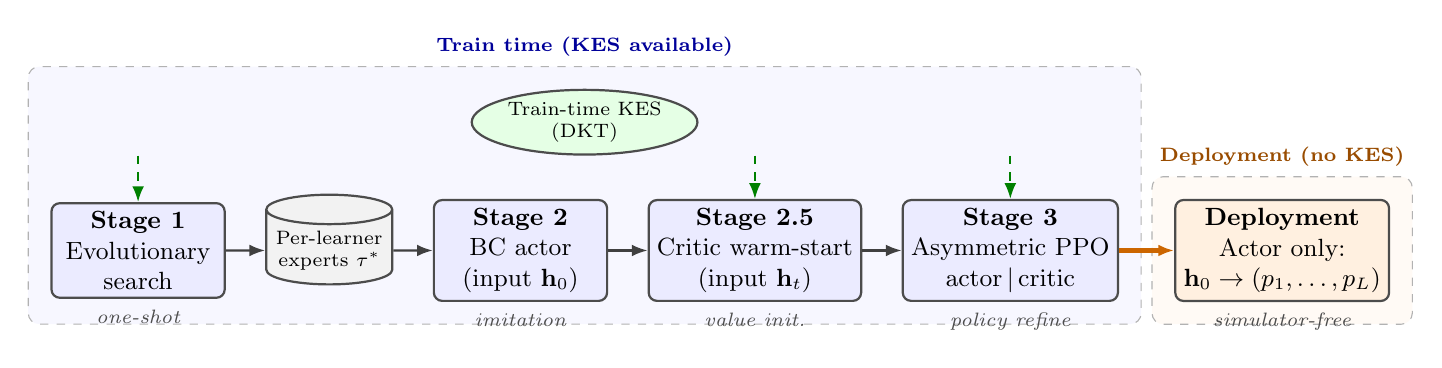
\begin{tikzpicture}[
        font=\small,
        stage/.style={rectangle, rounded corners=3pt, draw=black!70, thick,
                      minimum width=2.2cm, minimum height=1.05cm, align=center,
                      fill=blue!8, inner sep=3pt},
        deploy/.style={rectangle, rounded corners=3pt, draw=black!70, thick,
                      minimum width=2.4cm, minimum height=1.05cm, align=center,
                      fill=orange!12, inner sep=3pt},
        data/.style={cylinder, shape border rotate=90, aspect=0.25, draw=black!70,
                     thick, fill=gray!10, minimum height=0.9cm, minimum width=1.6cm,
                     align=center, inner sep=2pt, font=\scriptsize},
        kes/.style={ellipse, draw=black!70, thick, fill=green!10,
                    minimum width=1.7cm, minimum height=0.7cm, align=center,
                    inner sep=1pt, font=\scriptsize},
        arr/.style={-{Latex[length=2mm]}, thick, black!75},
        kesarr/.style={dashed, -{Latex[length=2mm]}, thick, green!50!black},
        lbl/.style={font=\scriptsize\itshape, text=black!70}
    ]
        %--- Stage boxes ---
        \node[stage] (s1) {\textbf{Stage 1}\\Evolutionary\\search};
        \node[data, right=0.5cm of s1] (exp) {Per-learner\\experts $\tau^*$};
        \node[stage, right=0.5cm of exp] (s2) {\textbf{Stage 2}\\BC actor\\(input $\mathbf{h}_0$)};
        \node[stage, right=0.5cm of s2] (s25) {\textbf{Stage 2.5}\\Critic warm-start\\(input $\mathbf{h}_t$)};
        \node[stage, right=0.5cm of s25] (s3) {\textbf{Stage 3}\\Asymmetric PPO\\actor$\,|\,$critic};
        \node[deploy, right=0.7cm of s3] (dep) {\textbf{Deployment}\\Actor only:\\$\mathbf{h}_0 \to (p_1,\ldots,p_L)$};

        %--- KES box (above) ---
        \node[kes, above=0.55cm of s2.north east, xshift=-0.3cm] (kes) {Train-time KES\\(DKT)};

        %--- Arrows: pipeline ---
        \draw[arr] (s1) -- (exp);
        \draw[arr] (exp) -- (s2);
        \draw[arr] (s2) -- (s25);
        \draw[arr] (s25) -- (s3);
        \draw[arr, line width=0.7mm, orange!80!black] (s3) -- (dep);

        %--- KES dashed arrows down to stages that consult it ---
        \draw[kesarr] (kes.south -| s1.north) -- (s1.north);
        \draw[kesarr] (kes.south -| s25.north) -- (s25.north);
        \draw[kesarr] (kes.south -| s3.north) -- (s3.north);

        %--- Region backgrounds ---
        \begin{scope}[on background layer]
            \node[draw=black!30, dashed, rounded corners=4pt, fill=blue!3,
                  fit=(s1)(s3)(kes), inner sep=8pt, label={[font=\scriptsize\bfseries,
                  text=blue!60!black]above:Train time (KES available)}] (train) {};
            \node[draw=black!30, dashed, rounded corners=4pt, fill=orange!4,
                  fit=(dep), inner sep=8pt, label={[font=\scriptsize\bfseries,
                  text=orange!60!black]above:Deployment (no KES)}] (deploy) {};
        \end{scope}

        %--- Footnote-style labels under stages ---
        \node[lbl, below=0.02cm of s1] {one-shot};
        \node[lbl, below=0.02cm of s2] {imitation};
        \node[lbl, below=0.02cm of s25] {value init.};
        \node[lbl, below=0.02cm of s3] {policy refine};
        \node[lbl, below=0.02cm of dep] {simulator-free};
    \end{tikzpicture}
    \caption{Overview of \ours{}. The KES (dashed green arrows) is consulted only at train time. \textbf{Stage~1} runs evolutionary search inside the KES to synthesize per-learner expert paths $\tau^*$. \textbf{Stage~2} distills $\tau^*$ into a feed-forward actor that consumes only the initial mastery $\mathbf{h}_0$ (deployment-realistic input). \textbf{Stage~2.5} warm-starts the critic on the privileged evolving mastery $\mathbf{h}_t$. \textbf{Stage~3} refines the actor with asymmetric PPO: the actor remains constrained to $\mathbf{h}_0$, while the critic continues to exploit $\mathbf{h}_t$. At \textbf{Deployment}, the actor alone emits the full $L$-step path; no KES query is needed.}
    \label{fig:framework}
\end{figure*}
%% ============================================================

\ours{} has three training stages (Figure~\ref{fig:framework}). All three rely on the KES for evaluation, but the deployed policy is simulator-free: only the actor network is shipped, and at inference it consumes the initial mastery $\mathbf{h}_0$ and target mask $\mathbf{g}$ to emit a full $L$-step path in a single forward pass per step.

\subsection{Stage 1: Evolutionary Expert Generation}
\label{sec:method_stage1}

For each training learner with history $\mathcal{H}$, targets $\mathcal{G}$, and initial mastery $\mathbf{h}_0$, we search for high-quality learning paths using an evolutionary algorithm.

\textbf{Candidate Space.} We construct a candidate set $\mathcal{C}$ of size at most $C$ by combining the target concepts, their prerequisites and similar concepts from the concept graph, and zone-of-proximal-development (ZPD) concepts whose mastery is closest to 0.5:
\begin{equation}
    \mathcal{C} = \mathcal{G} \cup \bigcup_{g \in \mathcal{G}} \left(\text{prereq}(g) \cup \text{sim}_K(g)\right) \cup \text{ZPD}.
\end{equation}

\textbf{Evolutionary Search.} We maintain a population of $N_{\text{pop}}$ candidate paths, each of length $L$ drawn from $\mathcal{C}$. Over $N_{\text{gen}}$ generations, the population evolves through tournament selection, ordered crossover, and point mutation. The fitness of each path $\mathbf{p}$ is evaluated in the KES:
\begin{equation}
    f(\mathbf{p}) = \ep(\mathcal{H}, \mathbf{p}, \mathcal{G}).
\end{equation}

\textbf{Expert Selection.} From the final population, we select the single best path per learner ($K=1$), yielding one expert trajectory per training learner. We find that selecting the highest-fitness path produces cleaner training signal for BC compared to diverse multi-path selection: with $K>1$ paths per learner, the same state maps to multiple conflicting actions, creating label noise that caps BC accuracy at $\sim$70\%. With $K=1$, each state has a unique target action, enabling sharper policy initialization.

\subsection{Stage 2: Behavioral Cloning}

The evolutionary expert trajectories provide state--action pairs for supervised learning. Consistent with the simulator-free actor design (Section~4.3), the BC state uses the initial mastery $\mathbf{h}_0$, ensuring the actor never depends on KES feedback during BC training, PPO fine-tuning, or inference. For each expert $(\mathbf{h}_0, \mathcal{G}, \mathbf{p}, \text{EP})$, we construct $L$ training examples:
\begin{equation}
    \{(\mathbf{s}_t, a_t)\}_{t=0}^{L-1}, \quad \mathbf{s}_t = [\mathbf{h}_0 \| \mathbf{g} \| t/L],
\end{equation}
where $\mathbf{g} \in \{0,1\}^M$ is the target mask, $t/L$ provides step position, and $a_t = p_t$ is the expert's action at step $t$. The step index and the used-concept exclusion mask (applied during action selection) are the only signals that differentiate steps, so the actor learns to plan an entire path from the initial knowledge state alone.

The policy $\pi_\theta$ is trained to minimize the cross-entropy loss:
\begin{equation}
    \mathcal{L}_{\bc} = -\frac{1}{|\mathcal{D}|} \sum_{(\mathbf{s}, a) \in \mathcal{D}} \log \pi_\theta(a \mid \mathbf{s}).
\end{equation}
The BC optimizer updates only the actor parameters; the critic head is trained separately in Stage~2.5 because its target distribution (privileged $\mathbf{h}_t$) differs from the actor's deployment distribution (blind $\mathbf{h}_0$).

\subsection{Stage 2.5: Critic Warm-Start}
\label{sec:critic_ws}

The PPO critic estimates $V(\mathbf{s}_t^{\text{critic}})$ where $\mathbf{s}_t^{\text{critic}}$ contains the evolving mastery $\mathbf{h}_t$ (Section~4.4). Initializing this head from scratch wastes early PPO updates on critic learning before useful advantage estimates appear. We therefore warm-start the critic on the expert trajectories: for each expert path we roll out the KES, compute the discounted return $G_t = \gamma^{L-1-t}\,\text{EP}$ at every step, and fit $V$ by mean-squared regression to $G_t$. The actor parameters are frozen during this stage.

\subsection{Stage 3: PPO Fine-Tuning}

Starting from the BC-initialized policy, we apply PPO~\cite{schulman2017ppo} for online fine-tuning. At each episode, we sample a batch of learners and collect trajectories by interacting with the KES.

\textbf{Simulator-Free Inference via Asymmetric Actor-Critic.}

A critical design consideration in KES-based LPR is whether the policy may access the simulator at inference time. As noted by Lee et al.~\cite{li2024privileged}, the simulator's internal knowledge state is unavailable in real deployment---a tutoring system cannot observe how a student's mastery evolves before they actually practice. Relying on per-step simulator feedback during inference is akin to planning a study schedule while already knowing the exam answers.

We address this through an asymmetric actor-critic architecture. The \textbf{actor} (policy) receives only the initial mastery $\mathbf{h}_0$ at every step, ensuring KES-free inference:
\begin{equation}
    \mathbf{s}_t^{\text{actor}} = [\mathbf{h}_0 \| \mathbf{g} \| t/L], \quad a_t \in \mathcal{K} \setminus \{a_0, \ldots, a_{t-1}\},
\end{equation}
where $\mathbf{g} \in \{0,1\}^M$ is the target mask and $t/L$ provides step position. The actor distinguishes steps through the step index and the used concept mask that excludes previously selected concepts from the action space. At deployment, the complete path is generated by $L$ forward passes through the actor alone, without simulator access.

The \textbf{critic} (value function), used only during training, receives the privileged evolving mastery $\mathbf{h}_t$ from the KES:
\begin{equation}
    \mathbf{s}_t^{\text{critic}} = [\mathbf{h}_t \| \mathbf{g} \| t/L].
\end{equation}
This asymmetry allows the critic to provide more accurate advantage estimates by observing how each recommendation affects mastery, while the actor learns to plan without this privileged information. The actor-critic separation ensures the deployed policy is fully simulator-free: it takes a learner's initial knowledge state and target concepts as input, and outputs a complete learning path in a single pass.

\textbf{Reward.} We use a sparse terminal reward computed via KES simulation:
\begin{equation}
    R_t = \begin{cases} \ep(\mathcal{H}, \mathbf{p}_{0:L}, \mathcal{G}) & \text{if } t = L-1 \\ 0 & \text{otherwise} \end{cases}
\end{equation}

\textbf{Policy Optimization.} The PPO clipped surrogate objective is:
\begin{equation}
    \mathcal{L}_{\ppo} = -\E_t\left[\min\left(\rho_t \hat{A}_t,\ \text{clip}(\rho_t, 1\pm\epsilon) \hat{A}_t\right)\right],
\end{equation}
where $\rho_t = \pi_\theta(a_t|\mathbf{s}_t^{\text{actor}}) / \pi_{\theta_{\text{old}}}(a_t|\mathbf{s}_t^{\text{actor}})$ is the importance ratio and $\hat{A}_t = R_t + \gamma V(\mathbf{s}_{t+1}^{\text{critic}}) - V(\mathbf{s}_t^{\text{critic}})$ uses the privileged critic. The full loss includes a value function term and an entropy bonus:
\begin{equation}
    \mathcal{L} = \mathcal{L}_{\ppo} + c_v \cdot \mathcal{L}_{\text{value}} - c_e \cdot H[\pi_\theta].
\end{equation}

\subsection{Expert-Utilization Variants}
\label{sec:variants}

Stages~2 and~3 above describe \ours{}-BC, the canonical instantiation. The downstream learner that consumes the evolutionary experts is, however, a design choice. We therefore consider two additional variants drawn from the sim-to-real literature:

\textbf{\ours{}-AWR.} Following Peng et al.~\cite{peng2019awr}, we replace Stage~2 with advantage-weighted regression. Each expert sample $(\mathbf{s},a)$ is weighted by $\exp(\hat{A}(\mathbf{s},a)/\beta)$, where the advantage is computed against a jointly updated value baseline. AWR up-weights expert actions whose realized return exceeds the baseline, making it a natural choice when experts have heterogeneous quality.

\textbf{\ours{}-DAPG.} Following Rajeswaran et al.~\cite{rajeswaran2018dexterous}, we keep Stage~2 as BC but replace Stage~3 with PPO augmented by a decaying BC term: $\mathcal{L} = \mathcal{L}_{\ppo} + \lambda_k\,\mathcal{L}_{\bc}^{\text{demo}}$ with $\lambda_k = \lambda_0\, \lambda_1^k$. This keeps the policy tethered to demonstrations early in PPO and gradually releases it.

All three variants share Stages~1 and~2.5 and differ only in how the expert distribution is exploited downstream. Section~6.2 shows that they converge to essentially the same EP, isolating the evolutionary expert synthesis as the operative mechanism rather than any particular imitation strategy.

%% ============================================================
\section{Experiments}
%% ============================================================

\subsection{Datasets}

We evaluate on three educational datasets that span the typical concept-count range of LPR studies (39--189 KCs):

\begin{itemize}
    \item \textbf{ASSIST15}~\cite{feng2009assistments}: An online mathematics tutoring platform. After filtering learners with $\geq$10 interactions, it contains 14,567 learners across 100 skill-builder concepts and 682K interactions.
    \item \textbf{Junyi Academy}~\cite{chang2015junyi}: an online mathematics learning platform. We sample 20,000 learners (seed-controlled) over 39 knowledge concepts and 4.9M interactions.
    \item \textbf{EdNet-KT1}~\cite{choi2020ednet}: A large-scale English-learning dataset from Santa. We sample 50,000 learners over 189 knowledge tags (from the official EdNet-Contents metadata) and 7.5M interactions.
\end{itemize}

Following the CSEAL protocol~\cite{liu2019cseal}, each dataset is split 50/50 into $\mathcal{D}_{\text{Sim}}$ (DKT training) and $\mathcal{D}_{\text{Off}}$ (LPR training and evaluation); $\mathcal{D}_{\text{Off}}$ is further split 80/10/10 into training, validation, and test partitions. Splits are seed-controlled so the three random seeds we report induce different student populations.

\subsection{Baselines}

We compare against 8 baselines spanning four categories. Heuristic methods (Random, Rule-based, uniform target repetition) are described in the appendix; Table~\ref{tab:main} reports the most competitive heuristic (\textit{Target-repeat}, cyclic repetition of target concepts) as a reference point.

\begin{itemize}
    \item \textbf{Sequential models with the same supervision:} \textit{GRU4Rec}~\cite{hidasi2016gru4rec} and \textit{SASRec}~\cite{kang2018sasrec} are standard recurrent and transformer-based sequence models. We train them on the same evolutionary trajectories as \ours{}-BC so that they share the supervisory signal and differ only in the downstream learner; the comparison therefore isolates the contribution of RL fine-tuning beyond pure imitation.
    \item \textbf{RL from scratch:} \textit{PPO-vanilla}~\cite{schulman2017ppo} uses the same asymmetric actor-critic architecture as \ours{} but is initialized from random weights and receives no expert demonstrations. This isolates the contribution of evolutionary pre-exploration.
    \item \textbf{Graph-enhanced RL:} \textit{CSEAL}~\cite{liu2019cseal} (A2C with cognitive navigation), \textit{GEHRL}~\cite{li2023gehrl} (hierarchical RL with goal planning), and \textit{DLELP}~\cite{cheng2025knowlp} (PPO with a plateau-detection similarity agent and a DKT-derived concept graph).
    \item \textbf{LLM-enhanced:} \textit{KnowLP}~\cite{cheng2025knowlp} shares the DLELP architecture but replaces the DKT-derived concept graph with an LLM-constructed EDU-GraphRAG graph (TextGrad refinement + 3-vote self-consistency); the same P-Agent and graph-aware candidate mask are used at training and inference, so the only difference between DLELP and KnowLP is the source of the graph.
\end{itemize}

We also report the three expert-utilization variants of our method---\textit{\ours{}-BC}, \textit{\ours{}-AWR}, \textit{\ours{}-DAPG} (Section~\ref{sec:variants})---which share Stage~1 and differ only in how the experts are exploited downstream. All baselines and variants are re-implemented in a unified codebase. Table~\ref{tab:baseline_fidelity} summarizes which aspects of each baseline are preserved verbatim from the original publication and which are modified for fair comparison. Specifically, we replace inference-time KES queries with $\mathbf{h}_0$-only planning so that all methods produce deployment-realistic recommendations, and we equalize the policy network capacity across PPO-based methods (asymmetric actor-critic with hidden 256/512 for Junyi/ASSIST15--EdNet). We emphasize the scope of this comparison: we do not claim superiority over the original, inference-time simulator-querying versions of CSEAL/GEHRL/DLELP/KnowLP under their own assumptions. Rather, we compare all methods under the deployment-free constraint targeted by this paper---namely, that no KT query is available at inference time on the live student. The performance gap observed under this constraint is precisely the quantity practitioners face when deploying any of these methods without a runtime KES. $\mathbf{h}_0$-only inference is the deployment definition: a learner's future mastery is unknowable before practice, so any method reported under inference-time KES access is measuring a counterfactual oracle rather than a servable system.

\begin{table*}[t]
\centering
\caption{Baseline fidelity. ``Original'' columns preserve the published method; ``Adapted'' columns describe our changes for deployment-realistic, capacity-matched comparison.}
\label{tab:baseline_fidelity}
\small
\begin{tabular}{@{}l|cccc@{}}
\toprule
Method & Algorithm preserved & Reward preserved & \makecell{Inference uses KES\\(original)} & \makecell{Inference uses KES\\(ours)} \\
\midrule
GRU4Rec~\cite{hidasi2016gru4rec}    & yes (GRU)                 & N/A (BC on experts)       & no  & no \\
SASRec~\cite{kang2018sasrec}        & yes (transformer)         & N/A (BC on experts)       & no  & no \\
PPO-vanilla~\cite{schulman2017ppo}  & yes (PPO + clip)          & terminal EP               & N/A & no (asymmetric AC) \\
CSEAL~\cite{liu2019cseal}           & yes (A2C + cognitive nav) & EP                        & yes & no (h$_0$-only actor) \\
GEHRL~\cite{li2023gehrl}            & yes (hierarchical PPO)    & EP                        & yes & no (h$_0$-only actor) \\
DLELP~\cite{cheng2025knowlp}        & yes (PPO + plateau S-agent)& EP                        & yes & no (S-agent off in h$_0$ mode; graph-aware candidate mask retained) \\
KnowLP~\cite{cheng2025knowlp}       & yes (DLELP + LLM graph)   & EP                        & yes & no (graph is EDU-GraphRAG instead of DKT-derived) \\
\bottomrule
\end{tabular}
\end{table*}

\subsection{Implementation Details}

\textbf{KES.} We train a DKT model~\cite{piech2015dkt} with an LSTM backbone on $\mathcal{D}_{\text{Sim}}$ using the pyKT framework~\cite{liu2022pykt} with its standard configuration (embedding size 200, dropout 0.1, learning rate $10^{-3}$, batch size 256). Validation AUCs: ASSIST15 0.70, Junyi 0.74, EdNet 0.76.

\textbf{Concept Graph.} Prerequisite and similarity graphs are derived from the DKT's cross-concept influence matrix with thresholds $\tau \in\{0.25, 0.05, 0.15\}$ for ASSIST15, Junyi, EdNet respectively (chosen so that the average degree is comparable across datasets).

\textbf{Evolutionary Search.} Population $N_{\text{pop}} = 60$, generations $N_{\text{gen}} = 50$, candidate cap $C = 30$. The single best path per learner is retained ($K=1$); we discuss the implications of $K>1$ in Section~\ref{sec:method_stage1}. Wall-clock generation time on a single GPU: 8.4 minutes for Junyi (8000 learners), 31 minutes for ASSIST15 (5827 learners), 41 minutes for EdNet (19880 learners).

\textbf{Policy Network.} Asymmetric actor-critic with two separate two-layer MLPs of hidden width 512 (ASSIST15, EdNet) or 256 (Junyi). The actor consumes $[\mathbf{h}_0\,\|\,\mathbf{g}\,\|\,t/L]$; the critic consumes $[\mathbf{h}_t\,\|\,\mathbf{g}\,\|\,t/L]$.

\textbf{Training.} BC: 2,000 epochs with Adam ($\text{lr}=10^{-3}$, weight decay $10^{-4}$, batch 4096); critic warm-start: 1,000 epochs of MSE regression on expert returns. PPO fine-tune: 30,000 episodes, batch size 128, $\text{lr}=10^{-4}$, clip $\epsilon=0.15$, entropy coefficient 0.03, cosine learning-rate schedule, 4 inner PPO epochs per batch, gradient clip 0.5. PPO-vanilla uses the same hyperparameters but no BC initialization. All experiments are repeated with three seeds ($\{42, 123, 7\}$); we report mean$\pm$std throughout. Hardware: a single NVIDIA A40 GPU.

\subsection{Main Results}

Table~\ref{tab:main} presents the EP scores across all datasets and path lengths.
\textbf{Across-the-board superiority with widening margins.}
\ours{} is the best or second-best method in every one of the 27 cells (3 datasets $\times$ 3 path lengths $\times$ 3 variants), and at least one \ours{} variant attains the column-wise maximum in every cell. Against PPO-vanilla---the strongest baseline and the most architecturally comparable competitor, since both share the asymmetric actor-critic architecture and hyperparameters and differ only in the presence of evolutionary expert pre-training---the gain is consistently positive and grows with the difficulty of the problem: on ASSIST15 it widens from $+0.050$ at $L\!=\!5$ to $+0.110$ at $L\!=\!20$ ($+22\%$); on Junyi it grows from $+0.039$ at $L\!=\!5$ to $+0.048$ at $L\!=\!20$; on EdNet (the largest concept set, $M\!=\!189$) the gain remains substantial at every $L$ and the search space at $L\!=\!20$ alone exceeds $9.4\!\times\!10^{43}$ candidate paths. Crucially, the gap is statistically robust: per-student paired Wilcoxon comparisons against PPO-vanilla yield $p\!<\!10^{-100}$ on every cell, with paired-win rates of $73$--$82\%$ across cells. The robustness analyses (Sections~\ref{sec:cross_sim} and~\ref{sec:stochastic}) further show that the within-simulator gain is amplified under DKT-instance shift ($+0.072\!\to\!+0.091$) and preserved under all three stochastic response models---indicating that the gain reflects a genuinely better policy rather than a deterministic-single-DKT artifact.

\begin{table*}[t]
\centering
\caption{Test EP (mean{\scriptsize$\pm$std} over 3 seeds) across datasets and path lengths. Best in \textbf{bold}, second best \underline{underlined}.}
\label{tab:main}
\resizebox{\textwidth}{!}{%
\begin{tabular}{@{}cl|c|cc|c|ccc|c|ccc@{}}
\toprule
& & Heuristic & \multicolumn{2}{c|}{Sequential} & RL & \multicolumn{3}{c|}{Graph-enhanced RL} & LLM & \multicolumn{3}{c}{\textbf{Ours}} \\
Dataset & $L$ & Target & GRU4Rec & SASRec & PPO & CSEAL & GEHRL & DLELP & KnowLP & \ours{}-BC & \ours{}-AWR & \ours{}-DAPG \\
\midrule
\multirow{3}{*}{\shortstack[c]{\textbf{Junyi}\\{\scriptsize 39 KCs}}}
& 5  & +0.203{\scriptsize$\pm$.003} & +0.237{\scriptsize$\pm$.008} & +0.256{\scriptsize$\pm$.007} & +0.247{\scriptsize$\pm$.010} & +0.054{\scriptsize$\pm$.049} & +0.106{\scriptsize$\pm$.003} & +0.110{\scriptsize$\pm$.013} & +0.089{\scriptsize$\pm$.019} & \underline{+0.286}{\scriptsize$\pm$.003} & \textbf{+0.286}{\scriptsize$\pm$.000} & +0.285{\scriptsize$\pm$.005} \\
& 10 & +0.244{\scriptsize$\pm$.002} & +0.266{\scriptsize$\pm$.009} & +0.320{\scriptsize$\pm$.006} & +0.364{\scriptsize$\pm$.003} & +0.178{\scriptsize$\pm$.008} & +0.138{\scriptsize$\pm$.008} & +0.247{\scriptsize$\pm$.003} & +0.230{\scriptsize$\pm$.010} & \textbf{+0.390}{\scriptsize$\pm$.001} & +0.388{\scriptsize$\pm$.001} & \underline{+0.390}{\scriptsize$\pm$.001} \\
& 20 & +0.286{\scriptsize$\pm$.001} & $-$0.005{\scriptsize$\pm$.017} & +0.299{\scriptsize$\pm$.006} & +0.380{\scriptsize$\pm$.005} & +0.207{\scriptsize$\pm$.006} & +0.045{\scriptsize$\pm$.029} & +0.337{\scriptsize$\pm$.010} & +0.337{\scriptsize$\pm$.010} & \underline{+0.426}{\scriptsize$\pm$.002} & +0.420{\scriptsize$\pm$.002} & \textbf{+0.428}{\scriptsize$\pm$.002} \\
\midrule
\multirow{3}{*}{\shortstack[c]{\textbf{ASSIST15}\\{\scriptsize 100 KCs}}}
& 5  & +0.296{\scriptsize$\pm$.011} & +0.329{\scriptsize$\pm$.007} & +0.355{\scriptsize$\pm$.008} & +0.420{\scriptsize$\pm$.011} & +0.062{\scriptsize$\pm$.022} & +0.211{\scriptsize$\pm$.007} & +0.251{\scriptsize$\pm$.015} & +0.189{\scriptsize$\pm$.034} & +0.470{\scriptsize$\pm$.003} & \underline{+0.471}{\scriptsize$\pm$.005} & \textbf{+0.472}{\scriptsize$\pm$.004} \\
& 10 & +0.321{\scriptsize$\pm$.009} & +0.325{\scriptsize$\pm$.010} & +0.466{\scriptsize$\pm$.011} & +0.543{\scriptsize$\pm$.009} & +0.215{\scriptsize$\pm$.013} & +0.228{\scriptsize$\pm$.003} & +0.454{\scriptsize$\pm$.002} & +0.388{\scriptsize$\pm$.011} & \textbf{+0.614}{\scriptsize$\pm$.002} & +0.604{\scriptsize$\pm$.001} & \underline{+0.613}{\scriptsize$\pm$.003} \\
& 20 & +0.331{\scriptsize$\pm$.007} & +0.332{\scriptsize$\pm$.007} & +0.473{\scriptsize$\pm$.005} & +0.511{\scriptsize$\pm$.009} & +0.292{\scriptsize$\pm$.005} & +0.142{\scriptsize$\pm$.018} & +0.230{\scriptsize$\pm$.015} & +0.293{\scriptsize$\pm$.062} & \underline{+0.621}{\scriptsize$\pm$.000} & +0.619{\scriptsize$\pm$.003} & \textbf{+0.624}{\scriptsize$\pm$.001} \\
\midrule
\multirow{3}{*}{\shortstack[c]{\textbf{EdNet}\\{\scriptsize 189 KCs}}}
& 5  & +0.104{\scriptsize$\pm$.001} & +0.188{\scriptsize$\pm$.001} & +0.200{\scriptsize$\pm$.000} & +0.263{\scriptsize$\pm$.003} & +0.136{\scriptsize$\pm$.006} & +0.052{\scriptsize$\pm$.002} & +0.197{\scriptsize$\pm$.006} & +0.165{\scriptsize$\pm$.003} & \underline{+0.277}{\scriptsize$\pm$.002} & +0.276{\scriptsize$\pm$.002} & \textbf{+0.278}{\scriptsize$\pm$.002} \\
& 10 & +0.138{\scriptsize$\pm$.001} & +0.240{\scriptsize$\pm$.005} & +0.260{\scriptsize$\pm$.003} & +0.367{\scriptsize$\pm$.003} & +0.187{\scriptsize$\pm$.006} & +0.045{\scriptsize$\pm$.009} & +0.264{\scriptsize$\pm$.009} & +0.227{\scriptsize$\pm$.002} & \underline{+0.383}{\scriptsize$\pm$.003} & +0.379{\scriptsize$\pm$.003} & \textbf{+0.384}{\scriptsize$\pm$.003} \\
& 20 & +0.172{\scriptsize$\pm$.002} & +0.266{\scriptsize$\pm$.006} & +0.275{\scriptsize$\pm$.008} & +0.457{\scriptsize$\pm$.004} & +0.229{\scriptsize$\pm$.007} & $-$0.089{\scriptsize$\pm$.006} & +0.352{\scriptsize$\pm$.010} & +0.321{\scriptsize$\pm$.004} & \textbf{+0.475}{\scriptsize$\pm$.003} & +0.466{\scriptsize$\pm$.005} & \underline{+0.474}{\scriptsize$\pm$.004} \\
\bottomrule
\end{tabular}%
}
\end{table*}

\subsection{Convergence Analysis}

\begin{figure}[t]
    \centering
    \includegraphics[width=\columnwidth]{convergence.pdf}
    \caption{Validation EP during training on ASSIST15 ($L{=}20$, 3-seed mean). The \ours{} variants emerge from Stage~2 already at Val EP $\approx +0.42$; PPO-vanilla starts at $0$ and crosses the same level only around episode 6{,}000 before plateauing near $+0.51$. \ours{} continues to climb to $+0.62$ over the remaining 24{,}000 episodes.}
    \label{fig:convergence}
\end{figure}

\subsection{Component Ablations}
\label{sec:ablation_random}

To pinpoint which components of \ours{} contribute to the gain, we run three controlled ablations on ASSIST15 $L\!=\!10$ (3 seeds, mean$\pm$std), the same setting used by our mechanism (\S\ref{sec:pedagogical}) and robustness (\S\ref{sec:cross_sim}, \S\ref{sec:stochastic}) analyses.

\begin{table}[t]
\centering
\caption{Component ablations on ASSIST15 $L{=}10$. All variants share the same actor-critic architecture and hyperparameters; only the indicated component is removed or replaced. Mean$\pm$std over 3 seeds (729 test learners each, except Greedy which is eval-only on 200 learners).}
\label{tab:ablation_components}
\begin{tabular}{@{}lc@{}}
\toprule
Variant & Test EP \\
\midrule
\emph{Search strategy at Stage~1} \\
\quad Greedy 1-step lookahead (no learning) & +0.155{\scriptsize$\pm$.029} \\
\quad Random-path experts $\to$ BC                  & +0.354{\scriptsize$\pm$.011} \\
\quad Evolutionary search $\to$ BC                  & \textbf{+0.614}{\scriptsize$\pm$.003} \\
\midrule
\emph{Downstream learner} \\
\quad PPO-vanilla (no experts, no pretraining)      & +0.543{\scriptsize$\pm$.009} \\
\quad \ours{}-BC w/o critic warm-start (Stage~2.5)  & +0.591{\scriptsize$\pm$.003} \\
\quad \ours{}-BC (full, Stages~1--3)                & \textbf{+0.614}{\scriptsize$\pm$.003} \\
\bottomrule
\end{tabular}
\end{table}

\textbf{(a) Why evolutionary search?}
We compare three strategies for producing Stage-1 paths under identical candidate sets and budgets. (i) Greedy 1-step lookahead, the cheapest non-random baseline, selects at each step the concept that maximizes immediate EP improvement; it ignores joint structure and reaches only $+0.155$, far below PPO-vanilla. (ii) Random-path experts discard search entirely; BC on them reaches $+0.354$, well below PPO-vanilla ($+0.543$), so any source of demonstrations is not enough---bad demonstrations actively bias the policy. (iii) Evolutionary search, which performs non-myopic global selection over the joint $L$-step space within the same candidate set, reaches $+0.614$. The contrast between greedy and evolutionary ($+0.459$ EP) is particularly informative: it isolates the value of joint sequence optimization over greedy local choices, which is precisely the combinatorial structure that motivates LPR.

\textbf{(b) Without critic warm-start.}
Removing Stage~2.5 and letting PPO learn the critic from scratch produces a small but consistent drop across all three seeds (Table~\ref{tab:ablation_components}). The warm-started critic primarily stabilizes the early phase of PPO by providing reliable advantage estimates from episode one; the asymptotic improvement is therefore expected to be modest, while the early-phase stability is the practical benefit.

\textbf{(c) Imitation algorithm is interchangeable.}
Table~\ref{tab:main} shows that BC, AWR, and DAPG yield within 0.01 EP of each other across all nine $\langle\text{dataset},L\rangle$ cells. Combined with (a), this rules out any specific imitation algorithm as the source of the improvement and confirms that evolutionary expert quality is the operative variable.

Together, the three ablations form a clean causal story: BC alone is not enough (b), random experts are not enough (a), but evolutionary experts plus a warm-started asymmetric actor-critic together produce the full effect. No single component can be dropped without measurable loss.


%% ============================================================
\section{Analysis}
%% ============================================================

\subsection{Where the Improvement Comes From}

Table~\ref{tab:main} establishes that \ours{} surpasses every baseline in every condition, but the more interesting question is why. We answer it with three complementary observations.

\textbf{(i) Search space reduction.}
The number of distinct $L$-step paths is $\binom{M}{L}\cdot L!$, which grows rapidly with both the number of concepts and the path length, as shown in Table~\ref{tab:search_space}.

\begin{table}[t]
\centering
\caption{Combinatorial search space size across datasets and path lengths.}
\label{tab:search_space}
\small
\begin{tabular}{@{}lrrr@{}}
\toprule
$L$ & Junyi ($M{=}39$) & ASSIST15 ($M{=}100$) & EdNet ($M{=}189$) \\
\midrule
5  & $7.0\!\times\!10^{7}$  & $9.0\!\times\!10^{9}$  & $2.4\!\times\!10^{11}$ \\
10 & $1.6\!\times\!10^{14}$ & $6.3\!\times\!10^{19}$ & $7.6\!\times\!10^{22}$ \\
20 & $1.4\!\times\!10^{27}$ & $5.4\!\times\!10^{37}$ & $9.4\!\times\!10^{43}$ \\
\bottomrule
\end{tabular}
\end{table}

RL from scratch must explore this space by sampling from a uniform initial policy, receiving non-zero reward only when the entire $L$-step path happens to improve the targets. Evolutionary search, by contrast, evaluates complete paths and selects on fitness, so it locates high-EP regions inside the simulator using $N_{\text{pop}}\!\times\!N_{\text{gen}}\!=\!3{,}000$ evaluations per learner, irrespective of $M$ or $L$. Behavioral cloning then transfers the located regions to a feed-forward policy.

\textbf{(ii) Higher starting point, shorter trajectory.}
The convergence curve on ASSIST15 $L\!=\!20$ (Figure~\ref{fig:convergence}, 3-seed mean) makes the effect concrete. The BC stage reaches Val EP $\approx +0.42$ before any PPO episode is taken, whereas PPO-vanilla starts at $\approx 0$ and needs $\sim$6{,}000 episodes to reach the same level---an episode budget that would otherwise be spent purely on rediscovering what the evolutionary experts already encode. After 30{,}000 episodes, PPO-vanilla plateaus at Val EP $\approx +0.51$ while \ours{} settles at $\approx +0.62$, a gap that the per-student paired Wilcoxon test confirms is highly significant ($p\!<\!10^{-100}$, 77.1\% paired wins on 1{,}500 students for the matched Junyi $L\!=\!10$ setting). Crucially, the gap is not an artifact of any single $\langle\text{dataset}, L\rangle$ cell: it widens monotonically with $L$ across all three datasets (Table~\ref{tab:main}), exactly as expected because the search space grows super-exponentially while the BC initialization provides a near-constant head start.

\textbf{(iii) Mitigated distribution shift.}
Pure BC suffers from compounding error~\cite{ross2011dagger}: small action mistakes drive the policy into states absent from the demonstrations. In \ours{}, PPO fine-tuning explicitly trains on the policy's own state distribution, closing the gap that BC leaves open. The asymmetric critic accelerates this correction because it observes the privileged $\mathbf{h}_t$ and produces lower-variance advantage estimates, despite the actor being constrained to the deployment-realistic $\mathbf{h}_0$.

\subsection{The Imitation Method Is Not the Mechanism}

A natural concern is whether the gain comes from a particular imitation algorithm rather than from the experts themselves. Table~\ref{tab:main} answers this directly: \ours{}-BC, \ours{}-AWR, and \ours{}-DAPG produce nearly indistinguishable final EP (within 0.01 across all nine $\langle\text{dataset},L\rangle$ conditions). AWR's advantage weighting and DAPG's decaying BC loss add no measurable benefit over plain BC.

To verify that the gains come specifically from evolutionary experts rather than from any source of demonstrations, we run an additional ablation in which the evolutionary path is replaced by a random permutation of $L$ distinct concepts (Section~\ref{sec:ablation_random}). All other components are kept identical. If imitation alone were enough, this random-expert variant would still benefit from BC initialization; the empirical result is the opposite.

\subsection{Pedagogical Coherence: Coverage and Sequencing}
\label{sec:pedagogical}

The improvement of \ours{} over PPO-vanilla can be decomposed along two pedagogically meaningful axes: what concepts are recommended and in what order they are arranged. To quantify these axes, we measure target coverage, defined as the fraction of target concepts appearing in the recommended path, and sequencing impact, defined as the drop in EP after uniformly shuffling the recommended path. The latter directly probes whether a path's effectiveness depends on ordering, which is a hallmark of pedagogically meaningful sequencing. Table~\ref{tab:pedagogical} reports the resulting decomposition.


\begin{table}[t]
\centering
\caption{Pedagogical decomposition on ASSIST15 $L\!=\!10$ (3 seeds, 200 test learners). ``EP$_\text{shuf}$'' is the average EP after uniformly shuffling each recommended path (5 shuffles per path); ``SeqDrop'' = EP$-$EP$_\text{shuf}$ measures the portion of EP that depends on \emph{ordering}.}
\label{tab:pedagogical}
\small
\begin{tabular}{@{}lccccc@{}}
\toprule
Method & EP & Coverage $\uparrow$ & EP$_\text{shuf}$ & SeqDrop $\uparrow$ & StepLift $\uparrow$ \\
\midrule
CSEAL          & +0.220 & 0.625 & +0.063 & +0.157 & +0.010 \\
GEHRL          & +0.252 & 0.784 & +0.070 & +0.182 & +0.011 \\
DLELP          & +0.479 & 0.435 & +0.213 & +0.266 & +0.017 \\
PPO-vanilla    & +0.561 & 0.713 & +0.333 & +0.227 & +0.020 \\
\midrule
\ours{}-BC     & \textbf{+0.627} & \textbf{0.876} & +0.330 & +0.297 & \textbf{+0.022} \\
\ours{}-AWR    & +0.616          & 0.864          & +0.327 & +0.289 & +0.022 \\
\ours{}-DAPG   & +0.625          & 0.861          & +0.327 & \textbf{+0.298} & +0.022 \\
\bottomrule
\end{tabular}
\end{table}

\textbf{Coverage.}
\ours{} variants recommend the target concepts at a substantially higher rate (0.86--0.88) than PPO-vanilla (0.71) and the graph-enhanced methods (0.44--0.78). Although coverage alone is not sufficient, since a random path that always contains the targets would not necessarily improve their mastery, it reflects a basic pedagogical requirement: the recommended sequence should expose the learner to the goals.

\textbf{Sequencing accounts for the entire \ours{}$-$PPO gap.}
Shuffling each method's path uniformly and re-evaluating yields EP$_\text{shuf}$ values that are essentially identical for \ours{}-BC ($+0.330$) and PPO-vanilla ($+0.333$). The two methods therefore select concept sets of indistinguishable quality, and the entire EP gap (+0.066) is recovered by the sequencing component (SeqDrop: \ours{} $+0.297$ vs.\ PPO $+0.227$, $\Delta=+0.070$). Graph-enhanced baselines (CSEAL, GEHRL) start from much lower-quality sets (EP$_\text{shuf}$ around $+0.07$), reflecting a different failure mode: weak concept selection rather than weak ordering. \ours{}'s evolutionary expert distillation is therefore best described as transferring an \emph{ordering policy} that PPO-vanilla cannot recover under sparse terminal reward; the per-step target lift (StepLift) is only marginally higher ($+0.022$ vs.\ $+0.020$).

This decomposition aligns with the well-known difficulty of credit assignment in sparse-reward RL: with a single terminal reward at step $L$, gradient updates cannot pinpoint which intermediate ordering decision was responsible. Evolutionary search bypasses this difficulty by evaluating complete trajectories end-to-end, so the experts encode order-sensitive structure that the policy then absorbs through imitation.


\subsection{Robustness to Simulator-Instance Shift}
\label{sec:cross_sim}

A natural concern with simulator-based training is that the learned policy might memorize idiosyncrasies of the specific KT instance used during training. To probe this, we keep each policy (and the state estimator, the original DKT trained with seed 42) fixed, and execute the recommended path against five alternative DKTs trained from scratch with seeds $\{7, 100, 200, 333, 999\}$ on different training subsets of $\mathcal{D}_{\text{Sim}}$. All alternative DKTs share the same architecture and hyperparameters (emb 200, dropout 0.1) as the original and reach comparable validation AUC ($0.700$--$0.708$ vs $0.704$), but encode different per-concept mastery dynamics (per-student Spearman rank correlation $0.62$). We restrict this stress test to within-DKT-family shift, i.e., alternative DKT instances trained with different random seeds and training subsets. This provides a controlled way to measure robustness to simulator variation caused by training data and initialization, which is the most direct source of simulator sensitivity in the standard KES-based LPR protocol.
\begin{table*}[t]
\centering
\caption{Robustness to DKT-instance shift on ASSIST15 $L\!=\!10$. Policies (3 seeds) trained against the original DKT (seed 42) are evaluated by executing their recommended paths on four alternative DKT instances with different training seeds (same architecture and hyperparameters). The state estimator is the original DKT throughout; only the execution simulator changes. All entries are means across 3 policy seeds $\times$ 200 test learners (same subset and evaluator as Table~\ref{tab:stochastic}, so the Original DKT column numbers differ from Table~\ref{tab:main} (729 learners) by at most $\pm 0.02$ EP per method). Methods are grouped by paradigm and, within each group, sorted by the cross-instance mean (descending). \textbf{Bold} marks the overall best per column.}
\label{tab:cross_sim}
\small
\setlength{\tabcolsep}{5pt}
\begin{tabular}{@{}lccccccc@{}}
\toprule
& & \multicolumn{4}{c}{\emph{Alternative DKT (different training seed)}} & & \\
\cmidrule(lr){3-6}
Method & Original DKT & seed 7 & seed 100 & seed 200 & seed 333 & \textbf{Mean (4 alts)} & $\Delta$ vs PPO \\
\midrule
\multicolumn{8}{@{}l}{\textit{\textbf{Simulator-guided demonstration learning (Ours)}}} \\
\quad \ours{}-BC   & \textbf{+0.630} & \textbf{+0.314} & \textbf{+0.337} & \textbf{+0.350} & +0.364          & \textbf{+0.341} & \textbf{+0.091} \\
\quad \ours{}-DAPG & +0.627          & +0.306          & +0.333          & +0.346          & +0.362          & +0.337          & +0.087 \\
\quad \ours{}-AWR  & +0.619          & +0.309          & +0.330          & +0.339          & \textbf{+0.367} & +0.336          & +0.086 \\
\midrule
\multicolumn{8}{@{}l}{\textit{Reinforcement learning baseline}} \\
\quad PPO-vanilla  & +0.558          & +0.219          & +0.270          & +0.240          & +0.269          & +0.250          & ---     \\
\midrule
\multicolumn{8}{@{}l}{\textit{Sequence recommenders}} \\
\quad SASRec       & +0.483          & +0.244          & +0.180          & +0.246          & +0.230          & +0.225          & $-$0.025 \\
\quad GRU4Rec      & +0.330          & +0.106          & +0.034          & +0.117          & +0.095          & +0.088          & $-$0.162 \\
\midrule
\multicolumn{8}{@{}l}{\textit{Knowledge-graph-based RL}} \\
\quad DLELP        & +0.471          & +0.258          & +0.184          & +0.212          & +0.206          & +0.215          & $-$0.035 \\
\quad GEHRL        & +0.246          & +0.045          & +0.001          & +0.054          & +0.035          & +0.034          & $-$0.216 \\
\quad CSEAL        & +0.211          & +0.057          & $-$0.020        & +0.053          & +0.017          & +0.027          & $-$0.223 \\
\midrule
\multicolumn{8}{@{}l}{\textit{LLM-enhanced graph-based RL}} \\
\quad KnowLP       & +0.299          & +0.134          & +0.141          & +0.191          & +0.141          & +0.152          & $-$0.098 \\
\bottomrule
\end{tabular}
\\[2pt]
{\footnotesize $\Delta$ vs PPO: difference in cross-instance mean against PPO-vanilla.}
\end{table*}

Four observations follow. First, all three \ours{} variants rank highest on all four alternative DKT instances, and their within-\ours{} variation (BC, AWR, DAPG within $\pm 0.005$ EP) is an order of magnitude smaller than the gap to any baseline. This indicates that the cross-instance advantage comes from evolutionary expert distillation rather than any specific downstream learner. Second, the method ranking is preserved across all four alternative instances: \ours{} $>$ PPO-vanilla $>$ SASRec $>$ DLELP $>$ KnowLP $>$ GRU4Rec $>$ \{GEHRL, CSEAL\}. The \ours{}-BC gap over PPO-vanilla widens from $+0.072$ on the original DKT to $+0.091$ on average across the alternatives. Third, the two pure graph-conditioned RL baselines (CSEAL, GEHRL) collapse to non-positive cross-instance EP, while PPO-vanilla, SASRec, DLELP, and KnowLP retain a sizable fraction of their within-instance EP; CSEAL and GEHRL pre-condition the policy on a graph derived from the \emph{specific} training DKT instance (cognitive navigation, high-level goal planner) and therefore lose precisely the structure they were trained to exploit once that simulator is replaced. KnowLP shows a milder degradation than CSEAL/GEHRL but still falls below PPO-vanilla on average ($\Delta = -0.098$): its LLM-built EDU-GraphRAG graph encodes semantic concept relations that transfer partially across DKT instances, but the resulting policy still selects more EP-incoherent concepts than methods (PPO, SASRec, DLELP) whose candidate structure is either learned end-to-end or aligned to the simulator family itself. In contrast, \ours{} derives experts directly from simulator states without conditioning on any fixed graph derivative, which explains the preserved ranking. This is not a hyperparameter artifact, since PPO-vanilla shares hyperparameters and capacity with \ours{} but does not exhibit comparable degradation. Fourth, absolute EP drops substantially when the execution simulator changes ($-0.27$ on average across all methods), reflecting DKT sensitivity to random seed rather than a policy-specific failure, with a uniform drop across all ten methods. This evidence quantifies robustness to DKT-instance shift within the standard KES-based LPR protocol, which uses DKT-family simulators~\cite{liu2019cseal,li2023gehrl,cheng2025knowlp}.

\subsection{Robustness to Stochastic Response Models}
\label{sec:stochastic}

A second concern specific to \ours{} is that Stage~1 optimizes EP directly inside the simulator, so the evolutionary search might exploit discontinuities introduced by the deterministic threshold $r\!=\!\mathbf{1}[h_c\!>\!0.5]$. We re-evaluate every trained policy (deterministic-trained checkpoints; no re-training) under three alternative response models that smooth out the threshold:
(i) \emph{Bernoulli}, $r\!\sim\!\mathrm{Bern}(h_c)$;
(ii) \emph{Slip/Guess (mild)}, $P(r{=}1)=(1{-}s)h_c + g(1{-}h_c)$ with $s\!=\!g\!=\!0.10$;
(iii) \emph{Slip/Guess (strong)}, the same with $s\!=\!g\!=\!0.20$.
Paths are deterministic ($\mathbf{h}_0$-only actors); only the response is randomized, with 20 stochastic rollouts per learner to reduce variance. The same perturbation is applied uniformly to all seven non-ours baselines (PPO-vanilla, SASRec, GRU4Rec, DLELP, KnowLP, GEHRL, CSEAL); the deterministic reference column uses the same 200-learner subset and the same evaluator code-path, so numbers differ from Table~\ref{tab:main} (729 learners) by at most $\pm 0.02$ EP.

\begin{table*}[t]
\centering
\caption{Robustness to stochastic response models on ASSIST15 $L\!=\!10$. The deterministic-trained checkpoint of each method is evaluated under Bernoulli and slip/guess response models without re-training (3 policy seeds $\times$ 200 test learners $\times$ 20 stochastic rollouts; $\mathbf{h}_0$-only paths). Methods grouped by paradigm and sorted within group by the mean across the three stochastic modes. \textbf{Bold} marks the overall best per column.}
\label{tab:stochastic}
\small
\setlength{\tabcolsep}{5pt}
\begin{tabular}{@{}lcccccc@{}}
\toprule
& & \multicolumn{3}{c}{\emph{Stochastic response model}} & & \\
\cmidrule(lr){3-5}
Method & Determ.\ (ref.) & Bernoulli & Slip/Guess (0.10) & Slip/Guess (0.20) & \textbf{Mean (3 stoch.)} & $\Delta$ vs PPO \\
\midrule
\multicolumn{7}{@{}l}{\textit{\textbf{Simulator-guided demonstration learning (Ours)}}} \\
\quad \ours{}-BC   & \textbf{+0.630} & \textbf{+0.305} & \textbf{+0.272} & +0.223          & \textbf{+0.267} & \textbf{+0.043} \\
\quad \ours{}-DAPG & +0.627          & +0.303          & +0.270          & \textbf{+0.224} & +0.266          & +0.042 \\
\quad \ours{}-AWR  & +0.619          & +0.302          & \textbf{+0.272} & +0.221          & +0.265          & +0.041 \\
\midrule
\multicolumn{7}{@{}l}{\textit{Reinforcement learning baseline}} \\
\quad PPO-vanilla  & +0.558          & +0.267          & +0.227          & +0.179          & +0.224          & ---     \\
\midrule
\multicolumn{7}{@{}l}{\textit{Sequence recommenders}} \\
\quad SASRec       & +0.483          & +0.146          & +0.125          & +0.094          & +0.122          & $-$0.102 \\
\quad GRU4Rec      & +0.330          & +0.009          & $-$0.014        & $-$0.039        & $-$0.015        & $-$0.239 \\
\midrule
\multicolumn{7}{@{}l}{\textit{Knowledge-graph-based RL}} \\
\quad DLELP        & +0.471          & +0.153          & +0.118          & +0.074          & +0.115          & $-$0.109 \\
\quad GEHRL        & +0.246          & $-$0.093        & $-$0.106        & $-$0.135        & $-$0.111        & $-$0.335 \\
\quad CSEAL        & +0.211          & $-$0.088        & $-$0.107        & $-$0.133        & $-$0.109        & $-$0.333 \\
\midrule
\multicolumn{7}{@{}l}{\textit{LLM-enhanced graph-based RL}} \\
\quad KnowLP       & +0.299          & $-$0.013        & $-$0.042        & $-$0.082        & $-$0.046        & $-$0.270 \\
\bottomrule
\end{tabular}
\\[2pt]
{\footnotesize $\Delta$ vs PPO: difference between the method's mean across the three stochastic modes and PPO-vanilla's mean. Bold entries identify the column-wise best across all ten methods.}
\end{table*}

Three observations are evident from Table~\ref{tab:stochastic}. First, all three \ours{} variants remain the top three methods under every stochastic response model, with within-\ours{} variation an order of magnitude smaller than the gap to PPO-vanilla (which is itself the strongest non-\ours{} method). The discontinuity-exploitation hypothesis would predict that EVOL's advantage should disappear once the threshold is smoothed; instead, the gap of \ours{}-BC over PPO-vanilla is preserved across all three stochastic models ($+0.038, +0.045, +0.044$ for Bernoulli, mild slip/guess, and strong slip/guess respectively, compared with $+0.072$ under the deterministic reference). Second, all methods incur a roughly comparable absolute drop when responses become stochastic ($-0.34$ to $-0.41$), reflecting that stochastic outcomes are intrinsically harder to optimize against than deterministic ones, irrespective of method. Third, the three graph-conditioned baselines (CSEAL, GEHRL, KnowLP) all turn non-positive under every stochastic response model, just as the two pure graph-conditioned baselines (CSEAL, GEHRL) did under DKT-instance shift, suggesting that any policy whose action set is shaped by a fixed concept graph loses traction when the simulator dynamics are perturbed. KnowLP transitions from cross-instance-robust ($+0.152$ in Table~\ref{tab:cross_sim}) to stochastic-fragile ($-0.046$ here, a $\Delta = -0.270$ deficit against PPO-vanilla), indicating that its LLM-built EDU-GraphRAG graph is calibrated to the deterministic threshold rather than to the underlying mastery dynamics, and degrades sharply once even mild response noise is introduced. Taken together, the two complementary stress tests (Sections~\ref{sec:cross_sim} and~\ref{sec:stochastic}) show that \ours{}'s advantage is preserved under both simulator-instance shift and response-model shift, and is therefore unlikely to stem from threshold or seed-specific shortcuts.

\subsection{Threats to Validity}
\label{sec:threats}

We discuss the principal threats to the validity of our claims and the evidence that mitigates each.

\textbf{Simulator-based evaluation protocol.}
Our evaluation follows the standard KES-based LPR protocol: a DKT model is trained as the knowledge evolution simulator, and learning paths are evaluated by the EP improvement induced inside this simulator~\cite{liu2019cseal,li2023gehrl,cheng2025knowlp}. This protocol is used by CSEAL, GEHRL, DLELP, and KnowLP, which makes it the appropriate controlled setting for comparing deployment-free LPR policies against prior KES-based methods. Under this protocol, every method is trained and evaluated against the same simulator interface, so the main comparison is fair and isolates the effect of the policy-learning method.

At the same time, simulator-based evaluation raises a natural concern: a method might overfit to the specific DKT instance used during training and evaluation. We therefore do not rely only on the original simulator. In Section~\ref{sec:cross_sim}, we perform an additional DKT-instance shift test by training alternative DKT simulators with different random seeds and training subsets, while keeping the recommendation policies fixed. This stress test asks whether a policy learned from one simulator still produces effective paths when the execution dynamics are changed within the same standard DKT-KES protocol. \ours{} remains the top-performing method on every alternative DKT instance, and its average gap over PPO-vanilla increases from $+0.072$ on the original DKT to $+0.091$ under DKT-instance shift. This suggests that the gain is not merely a single-simulator artifact. In contrast, several graph-conditioned baselines degrade sharply under the same shift, indicating that the evaluation is capable of exposing simulator-specific shortcuts rather than uniformly favoring all methods.

We also include two additional checks against simulator overfitting. First, the per-student paired Wilcoxon test against PPO-vanilla yields $p\!<\!10^{-100}$ on Junyi $L\!=\!10$, with \ours{} winning on 77.1\% of 1{,}500 students; this shows that the improvement is not driven by a small subset of easy cases. Second, replacing evolutionary experts with uniformly random paths collapses performance below PPO-vanilla (Table~\ref{tab:ablation_components}), ruling out the possibility that the gain comes simply from having any demonstration data. Together, these results support the interpretation that the benefit comes from high-quality per-learner expert synthesis rather than from exploiting one fixed simulator instance.

\textbf{Deterministic response model.}
Following the EduSim/CSEAL protocol~\cite{liu2019cseal}, the KES emits binary responses via deterministic thresholding, $r=\mathbf{1}[h_c>0.5]$. This rule is applied uniformly to every method during training and evaluation, so the main comparison remains controlled. However, because \ours{} uses evolutionary search to optimize paths inside the simulator, it is important to test whether the method exploits artifacts of this deterministic threshold.

We address this in Section~\ref{sec:stochastic} by evaluating the deterministic-trained checkpoints under three stochastic response models without retraining: Bernoulli responses and two slip/guess models. If \ours{} were relying on threshold-specific discontinuities, its advantage should disappear when responses are randomized. Instead, all three \ours{} variants remain the top-performing methods across all stochastic response models, and the gap over PPO-vanilla is preserved within $0.038$--$0.045$ EP. Thus, the advantage is not explained by deterministic-threshold exploitation.

\textbf{Deployment-free assumption.}
The paper targets one-shot, deployment-free LPR: the system must recommend the full path before the learner executes it. This assumption is stricter than inference-time simulator planning, where a method repeatedly simulates intermediate learner responses, appends them to the learner history, and chooses later concepts from the resulting counterfactual states. We adopt the stricter setting because it matches the information available to a deployed recommender: before the path begins, the system has access only to the learner's observed pre-path history and the initial mastery estimate derived from it.

This design choice may make some prior methods appear weaker than their original simulator-querying versions. We view this as a necessary consequence of evaluating a deployable policy rather than an oracle-style planner. To make the comparison fair, all baselines are adapted to the same $\mathbf{h}_0$-only inference constraint and, for PPO-based methods, comparable network capacity and training budgets are used. The reported gaps should therefore be interpreted as performance differences under deployment-realistic information access, not as claims about the original methods under their more permissive inference-time simulator assumptions.

\textbf{Pedagogical coherence.}
EP measures mastery improvement in the simulator and does not by itself guarantee that every recommended path satisfies all human-interpretable pedagogical constraints, such as a perfect prerequisite order. We therefore complement EP with a pedagogical decomposition in Section~\ref{sec:pedagogical}. The results show that \ours{} improves target coverage and, more importantly, gains over PPO-vanilla primarily through ordering: after shuffling the recommended paths, \ours{} and PPO-vanilla have nearly identical EP, while the original ordered paths differ substantially. This indicates that the evolved demonstrations transfer useful sequence structure rather than merely selecting easier concept sets. Nevertheless, we interpret this as evidence of improved order sensitivity, not as a guarantee of prerequisite-perfect curriculum design.

\subsection{Generalizability of the Recipe}

The proposed recipe is not tied to a particular dataset or a particular imitation objective. It requires three ingredients: (i) a simulator that can be queried during training, (ii) a combinatorial sequence decision problem with sparse terminal reward, and (iii) instance-specific optimal or near-optimal sequences that are difficult to obtain from human demonstrations. Educational learning path recommendation satisfies these conditions: the KES can evaluate candidate paths offline, the number of possible paths grows combinatorially with $M$ and $L$, and student logs record historical behavior rather than expert prescriptions.

Within this setting, \ours{} separates simulator use from deployment. The simulator is used offline to synthesize high-quality per-learner expert paths, and the resulting behavior is distilled into an actor that uses only deployable inputs at inference time. This separation is the central recipe: expensive or privileged search is allowed during training, but the deployed policy must act without simulator rollouts or counterfactual intermediate feedback. The same pattern can apply to other sequential recommendation problems where training-time simulators exist but deployment-time interaction must be planned in advance, such as personalized tutoring across curricula, treatment-sequence recommendation with patient simulators, or content-layout planning with user-response simulators.

%% ============================================================
\section{Conclusion}
%% ============================================================

In this work, we presented \ours{}, a simulator-guided demonstration-learning framework for deployment-realistic learning path recommendation. \ours{} addresses two coupled obstacles in KES-based LPR, namely blind sequential planning under sparse terminal reward and the absence of expert trajectories in educational data, by using the DKT-based simulator as a source of per-learner demonstrations synthesized through evolutionary search. These demonstrations are distilled into an asymmetric actor-critic whose actor plans from the initial mastery state alone, producing learning paths without KES queries at deployment. Across three datasets and three path lengths, \ours{} consistently outperforms eight baselines, and the near-identical performance of BC, AWR, and DAPG shows that the operative mechanism is evolutionary expert synthesis rather than the choice of imitation objective. The central bottleneck in deployment-realistic LPR is therefore not the imitation objective, but the synthesis of high-quality per-learner expert trajectories.

\section*{GenAI Usage Disclosure}

The authors used LLM-based tools only for writing assistance, including English drafting, grammar correction, and wording refinement. All AI-assisted content was reviewed and edited by the authors, who take full responsibility for the final manuscript.

%% ============================================================
%% References
%% ============================================================
\bibliographystyle{ACM-Reference-Format}
\begin{thebibliography}{25}

\bibitem{piech2015dkt}
C.~Piech, J.~Bassen, J.~Huang, S.~Ganguli, M.~Sahami, L.~Guibas, and J.~Sohl-Dickstein.
\newblock Deep knowledge tracing.
\newblock In \emph{Advances in Neural Information Processing Systems (NeurIPS)}, pages 505--513, 2015.

\bibitem{liu2019cseal}
Q.~Liu, S.~Tong, C.~Liu, H.~Zhao, E.~Chen, H.~Ma, and S.~Wang.
\newblock Exploiting cognitive structure for adaptive learning.
\newblock In \emph{Proceedings of the 25th ACM SIGKDD International Conference on Knowledge Discovery \& Data Mining (KDD)}, pages 627--635, 2019.

\bibitem{li2023gehrl}
Q.~Li, W.~Xia, L.~Yin, J.~Shen, R.~Rui, W.~Zhang, X.~Chen, R.~Tang, and Y.~Yu.
\newblock Graph enhanced hierarchical reinforcement learning for goal-oriented learning path recommendation.
\newblock In \emph{Proceedings of the 32nd ACM International Conference on Information and Knowledge Management (CIKM)}, pages 1318--1327, 2023.

\bibitem{cheng2025knowlp}
X.~Cheng, Z.~Zhang, J.~Wang, L.~Fang, C.~He, Q.~Guan, S.~Pan, and W.~Luo.
\newblock GraphRAG-induced dual knowledge structure graphs for personalized learning path recommendation.
\newblock \emph{arXiv preprint arXiv:2506.22303}, 2025.

\bibitem{chen2023src}
X.~Chen, J.~Shen, W.~Xia, J.~Jin, Y.~Song, W.~Zhang, W.~Liu, M.~Zhu, R.~Tang, K.~Dong, D.~Xia, and Y.~Yu.
\newblock Set-to-sequence ranking-based concept-aware learning path recommendation.
\newblock In \emph{Proceedings of the AAAI Conference on Artificial Intelligence}, 37(4):5027--5035, 2023.

\bibitem{schulman2017ppo}
J.~Schulman, F.~Wolski, P.~Dhariwal, A.~Radford, and O.~Klimov.
\newblock Proximal policy optimization algorithms.
\newblock \emph{arXiv preprint arXiv:1707.06347}, 2017.

\bibitem{hidasi2016gru4rec}
B.~Hidasi, A.~Karatzoglou, L.~Baltrunas, and D.~Tikk.
\newblock Session-based recommendations with recurrent neural networks.
\newblock In \emph{Proceedings of the 4th International Conference on Learning Representations (ICLR)}, 2016.

\bibitem{zhang2017dkvmn}
J.~Zhang, X.~Shi, I.~King, and D.-Y.~Yeung.
\newblock Dynamic key-value memory networks for knowledge tracing.
\newblock In \emph{Proceedings of the 26th International Conference on World Wide Web (WWW)}, pages 765--774, 2017.

\bibitem{pandey2019sakt}
S.~Pandey and G.~Karypis.
\newblock A self-attentive model for knowledge tracing.
\newblock In \emph{Proceedings of the 12th International Conference on Educational Data Mining (EDM)}, 2019.

\bibitem{ghosh2020akt}
A.~Ghosh, N.~Heffernan, and A.~S.~Lan.
\newblock Context-aware attentive knowledge tracing.
\newblock In \emph{Proceedings of the 26th ACM SIGKDD International Conference on Knowledge Discovery \& Data Mining (KDD)}, pages 2330--2339, 2020.

\bibitem{choi2020saint}
Y.~Choi, Y.~Lee, J.~Cho, J.~Baek, B.~Kim, Y.~Cha, D.~Shin, C.~Bae, and J.~Heo.
\newblock Towards an appropriate query, key, and value computation for knowledge tracing.
\newblock In \emph{Proceedings of the 7th ACM Conference on Learning @ Scale (L@S)}, pages 341--344, 2020.

\bibitem{choi2020ednet}
Y.~Choi, Y.~Lee, D.~Shin, J.~Cho, S.~Park, S.~Lee, J.~Baek, C.~Bae, B.~Kim, and J.~Heo.
\newblock EdNet: A large-scale hierarchical dataset in education.
\newblock In \emph{Proceedings of the 21st International Conference on Artificial Intelligence in Education (AIED)}, Part II, LNCS vol. 12164, pages 69--73. Springer, 2020.

\bibitem{feng2009assistments}
M.~Feng, N.~Heffernan, and K.~Koedinger.
\newblock Addressing the assessment challenge with an online system that tutors as it assesses.
\newblock \emph{User Modeling and User-Adapted Interaction}, 19(3):243--266, 2009.

\bibitem{chang2015junyi}
H.-S.~Chang, H.-J.~Hsu, and K.-T.~Chen.
\newblock Modeling exercise relationships in e-learning: A unified approach.
\newblock In \emph{Proceedings of the 8th International Conference on Educational Data Mining (EDM)}, pages 532--535, 2015.

\bibitem{chen2018prerequisite}
Y.~Chen, Q.~Liu, Z.~Huang, L.~Wu, E.~Chen, R.~Wu, Y.~Su, and G.~Hu.
\newblock Prerequisite-driven deep knowledge tracing.
\newblock In \emph{Proceedings of the IEEE International Conference on Data Mining (ICDM)}, pages 39--48, 2018.

\bibitem{ross2011dagger}
S.~Ross, G.~Gordon, and D.~Bagnell.
\newblock A reduction of imitation learning and structured prediction to no-regret online learning.
\newblock In \emph{Proceedings of the 14th International Conference on Artificial Intelligence and Statistics (AISTATS)}, pages 627--635, 2011.

\bibitem{torabi2018bc}
F.~Torabi, G.~Warnell, and P.~Stone.
\newblock Behavioral cloning from observation.
\newblock In \emph{Proceedings of the 27th International Joint Conference on Artificial Intelligence (IJCAI)}, pages 4950--4957, 2018.

\bibitem{jaderberg2017pbt}
M.~Jaderberg, V.~Dalibard, S.~Osindero, W.~M.~Czarnecki, J.~Donahue, A.~Razavi, O.~Vinyals, T.~Green, I.~Dunning, K.~Simonyan, C.~Fernando, and K.~Kavukcuoglu.
\newblock Population based training of neural networks.
\newblock \emph{arXiv preprint arXiv:1711.09846}, 2017.

\bibitem{salimans2017es}
T.~Salimans, J.~Ho, X.~Chen, S.~Sidor, and I.~Sutskever.
\newblock Evolution strategies as a scalable alternative to reinforcement learning.
\newblock \emph{arXiv preprint arXiv:1703.03864}, 2017.

\bibitem{khadka2018erl}
S.~Khadka and K.~Tumer.
\newblock Evolution-guided policy gradient in reinforcement learning.
\newblock In \emph{Advances in Neural Information Processing Systems (NeurIPS)}, pages 1196--1208, 2018.

\bibitem{rajeswaran2018dexterous}
A.~Rajeswaran, V.~Kumar, A.~Gupta, G.~Vezzani, J.~Schulman, E.~Todorov, and S.~Levine.
\newblock Learning complex dexterous manipulation with deep reinforcement learning and demonstrations.
\newblock In \emph{Proceedings of Robotics: Science and Systems (RSS)}, 2018.

\bibitem{nair2018demonstrations}
A.~Nair, B.~McGrew, M.~Andrychowicz, W.~Zaremba, and P.~Abbeel.
\newblock Overcoming exploration in reinforcement learning with demonstrations.
\newblock In \emph{IEEE International Conference on Robotics and Automation (ICRA)}, pages 6292--6299, 2018.

\bibitem{lange2023evosax}
R.~T.~Lange.
\newblock evosax: JAX-based evolution strategies.
\newblock In \emph{Proceedings of the Companion Conference on Genetic and Evolutionary Computation (GECCO)}, pages 659--662, 2023.

\bibitem{li2024evorl}
P.~Li, J.~Hao, H.~Tang, X.~Fu, Y.~Zheng, and K.~Tang.
\newblock Bridging evolutionary algorithms and reinforcement learning: A comprehensive survey on hybrid algorithms.
\newblock \emph{IEEE Transactions on Evolutionary Computation}, 2024.

\bibitem{li2024privileged}
Q.~Li, W.~Xia, L.~Yin, J.~Shen, R.~Rui, W.~Zhang, X.~Chen, R.~Tang, and Y.~Yu.
\newblock Privileged knowledge state distillation for reinforcement learning-based educational path recommendation.
\newblock In \emph{Proceedings of the 30th ACM SIGKDD Conference on Knowledge Discovery and Data Mining (KDD)}, 2024.

\bibitem{peng2019awr}
X.~B.~Peng, A.~Kumar, G.~Zhang, and S.~Levine.
\newblock Advantage-weighted regression: Simple and scalable off-policy reinforcement learning.
\newblock \emph{arXiv preprint arXiv:1910.00177}, 2019.

\bibitem{kang2018sasrec}
W.-C.~Kang and J.~McAuley.
\newblock Self-attentive sequential recommendation.
\newblock In \emph{IEEE International Conference on Data Mining (ICDM)}, pages 197--206, 2018.

\bibitem{liu2022pykt}
Z.~Liu, Q.~Liu, J.~Chen, S.~Huang, J.~Tang, and W.~Luo.
\newblock pyKT: A Python library to benchmark deep learning based knowledge tracing models.
\newblock In \emph{Advances in Neural Information Processing Systems (NeurIPS) Datasets and Benchmarks Track}, 2022.

\end{thebibliography}

\end{document}
